\taskpic{ От шара радиусом $R$, сделанного из органического стекла
  (показатель преломления $n$), осторожно отпиливают два маленьких
  кусочка так, что получаются две плосковыпуклые линзы --- диаметр
  первой составляет $d$, а диаметр второй вдвое больше. Линзы
  аккуратно склеивают плоскими поверхностями. На главной оптической
  оси этой системы на расстоянии 1 м от неё помещают точечный источник
  света, а с другой стороны --- экран. Как нужно его расположить,
  чтобы пятно на нём имело минимальный размер? Чему он равен? }
{
  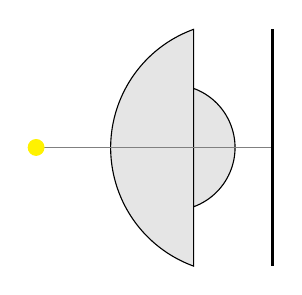
\begin{tikzpicture}
    \draw[fill=gray!20] (2,3) arc (110:250:1.6cm) -- cycle;
    \draw[fill=gray!20] (2,2.25) arc (70:-70:0.8cm) -- cycle;
    \draw[gray] (0,1.5) -- (3,1.5);
    \draw[very thick] (3,3) -- (3,0);
    \draw[yellow,fill=yellow] (0,1.5) circle (0.1cm);
  \end{tikzpicture}
}
% Квант, 2003-3, №1862